\chapter{Literature review}

\section{What is Autism?}

Autism is a life-long condition which affects how an individual may perceive and communicate to the world around them\cite{nas}. It is currently diagnosed by the presence of atypicalities in two domains: Restricted and Repetitive Behaviours(RRBs) and Social communication.

Firstly RRBs which entail insistence on sameness(IS) such as keeping strict routines and can come with distress with small changes, repetitive movements, flipping objects or echolalia and in addition encompasses sensory atypicalities \cite{dsm52}. These can lead to challenging behaviours defined as self-injurious, aggressive, inattention or disruptive behaviours\cite{teacherchallenge}, however the National Autistic Society suggested these behaviours are not stopped as they may serve unknown function,
 
The second domain is social communication and interaction deficits; an individual with autism may struggle with non-verbal ques such as body language, facial expressions, eye contact and understanding of gestures. In addition to adjusting behaviour in social contexts, difficulty in imaginative play or making friends.  

As a spectrum disorder, the range and severity of symptoms are unique to each person and thus a person with autism is classified into three different levels with the first requiring some support and the latter requiring substantial amounts\cite{dsm52}. Those on the low-functioning level of the spectrum, may have little to no verbal language and prefer to communicate using visual mediums such as PECS. For those with autism on the high-functioning side of the spectrum(i.e Aspergers) their difficulties can be less obvious; they may develop superb language skills but have difficulty using these in a social context which may lead to unintentional social offence or ridicule. Deficits with social imagination and theory of mind create difficulty in seeing another person's perspective and can lead to miscommunication and misinterpretation. 

With some of the disadvantages that may come with having autism, there are reported strengths that arise from their unique cognitive style i.e a talent for spotting details\cite{bayes} or having an impeccable memory of facts in relation to their 'special interests'. This further gives rise to the notion that Autism is not a disability, but a cognitive difference with it's own set of positives and negatives. 

In the last decade there has appeared to be improvements in public perception and understanding of autism and other cognitive differences such as Dyslexia and ADHD but there is still much left to be desired. Figures drawn from the 2011 census estimate that 1.1\% of the population have Autism\cite{nas} and as this figure has greatly risen\cite{increasingprevalence} so too has the need for greater public awareness and understanding\cite{autism_awareness} resulting in millions of pounds being spent on campaigns across the globs, such as World Autism Awareness Day and Light it up blue organised by Autism speaks(2013)\cite{autism_awareness}. 

A survey published by the National Autistic Society revealed that 92\% of respondents had heard of Autism but only 48\% had heard of Aspergers syndrome which has less obvious difficulties. Research has indicated that general members of the public are aware of communication and social issues that come with autism\cite{autismmisconception}, but little are aware of sensory difficulties\cite{autism_awareness}. In \cite{autism_awareness}, of 1204 people surveyed, 293 were aware of communication difficulties, 131 social but only 12 were aware of sensory difficulties. These is alarming owing "Many people with Asperger syndrome/High functioning autism define their sensory processing problems as more disabling than the deficits in communication/social behaviour\cite{olgab}.

\begin{quote}
If I could make one change... every person who comes into contact with my daughter would have some form of training in autism.\cite{nasschool}
\end{quote}

\section{Sensory Experiences}
Sensory processing differences in autism are highly reported, 81\% of respondents reported differences in visual perception, 87\% in hearing, 77\% in tactile perception, 30\% in taste and 56\% in smell \cite{sensory_leisure}. Senses play a vital role in how we model and perceive the world around and differing sensory experiences can result in differing views and behaviours.
 
Senses in autism can be hyper(more sensitive), hypo(less sensitive), agnostic or fluctuate between hyper and hypo\cite{bayes}. Fluctuations can be described as a "FM radio that is not exactly tuned on the station when you are driving down the freeway. Sometimes the world comes in clearly and at other times it does not" \cite{olgab}. As with all areas of autism, sensory atypicalities are unique to each individual, however, fluctuations can create a particular challenge for the individual and for carers in being able to predict troubling sources before they occur. 

When a sensory channel is in a state of agnosia, although able to see, one may not be able to assign it to any meaning, the individual becomes 'mind-blind', or 'mind-deaf' and consequently act as if they are genuinely deaf or blind. Below are examples of the effects someone with autism may experience depending on the state of their sensory channel:

\begin{table}[H]
    \begin{tabular}{| l | p{5cm} | p{5cm} |}
    \hline
    Sense channel & Hyper                                                                                                                      & Hypo                                                                   \\
    \hline
    \hline
    Vision        & Vision may be magnified                                                                                                    & Attracted to light or fascinated with bright colors                    \\
    \hline
    Auditory      & Sounds are amplified. Temple Grandin a write with autism described her ears as like 'microphones'                          & Is attracted to sounds/noises                                          \\
    \hline
    Tactile       & Clothes may hurt. One person with autism described clothe labels as feeling like 'barbed wire'. May not like being hugged. & Enjoys being hugged or seeks pressure by crawling under heavy objects. \\
    \hline
    Taste/Smells & Smells or texture of foods may be intolerable. & Mouths and licks objects \\
    \hline
    Vestibular & Difficulty with walking or crawling on uneven or unstable surfaces. & Spins, runs round and round, rocks back and forth \\
    \hline
    \end{tabular}
\end{table}

Sensory or information overloads can be the result of information coming in too fast and too quickly to be processed and although these are not unique to autism, it is a highly prevalent feature. For some, sensory overloads may not be caused by the stimuli itself, but the amount of stimuli and channels required, the sudden unpredictable onset or the type i.e high pitched noises rather than the volume or unpredictability of stimuli. "High sounds like sirens and whistles hurt my ears, and sudden sounds like a car horn and loud sounds, booming sounds like waves on the beach and roaring sounds like a vacuum cleaner or lawn mower". 

Distortions are reported to become worse in the state of nervous over-arousal and information overloads\cite{olgab} thus a cyclic problem emerges with an individual being more susceptible under stress; the more stressed the more they occur and the more stressed they become. Sensory overloads caused by sounds have been attributed to causing visual distortions, misconceptions on depth and distance causing disorientation\cite{sensoryexperiences} as overloads in one sense can cause issues with another. "Sensory overload caused by bright lights, fluorescent lights, colours, and patterns makes the body react as if being attacked or bombarded, resulting in such physical symptoms as headaches, anxiety, panic attacks or aggression"\cite{bayes}. 

Coping tools developed include learning to predict the causes, learning to avoid them or withdrawing into ones own quiet and peaceful world. Additionally, the effects can be reduced by concentrating on another specific sense, utilizing mono-processing and drowning out all other stimulus. 

Correlation found between sensory difficulties, difficult temperament characteristics, adaptability to changing context, quality of mood, threshold of responsiveness, intensity of reaction and persistence\cite{temperament}. Challenging behaviours may result from attempting to deal with adverse sensory effects. Spinning and rocking may be used as a means of inducing a positive sensory stimuli experience with desire for strict routines used to help deal with the worlds unpredictable nature\cite{sensory_overview}. When senses are in a hypo state, an individual may attempt to kick start their sensory system by banging on doors, hitting ears or self-injurious behaviour\cite{sensory_overview}. 

It was found that 40\% of children with autism had unusual fears in comparison to 0-5\% of typical children and the vast majority of these fears consisted of mechanical objects. Children with autism have higher levels of anxiety than typical children\cite{fears} and increased anxiety from being faced with more fears on a day to day basis will only increase stress. "The fear that it might happen can be as bad as it actually happening"\cite{fears} and even if the cause is identified and removed, for example not flushing the toilet whilst the child is in the bathroom, it can take considerable time for the worry to go away.

Perceived unusual fears could include leaving the house because it's cloudy and a fear of rain, not taking a shower because of the noise from the drain, not going to school due to being afraid the fire alarm will sound. The top five reported unusual fears were toilets, elevators, vacuum cleaners, thunderstorms, tornadoes. The cause of many of these unusual fears in children with autism are thought to be related to sensory perception differences\cite{fears}.

\section{Theoretical models}
Many theories of the potential causes of autism posit it as the result of a complex information processing disorder\cite{minshewmodel}. Many theoretical models of autism that have been put forward to describe not only the deficits associated with autism but also their reported strengths. People with autism are shown to have greater skills in areas such as EFT(Embedded Figure Tests) which require an individual to identify a shape in a more complex image in addition abilities to naturally spot details and patterns. The theoretical models give indication of potential causes of sensory overloads and why some challenging behaviours may result. These models give further weight to the idea that autism is not a disability but the result of a difference in information processing and cognitive style. 

\subsection{Information processing}

It is suggested that people with autism process information holistically, a theory known as Gestalt perception. Gestalt perception is posited to cause fragmented or distorted perceptions in people with autism\cite{olgab}; processing information as a whole instead of in parts make it difficult to drawn connections and thus make predictions about the world. When one small detail in the environment changes the gestalt changes meaning a previously recognisable environment is looked upon as new. Routines may be used as one method to alleviate this.

"I had always known that the world was fragmented. My mother was a small and a texture, my father was a tone, and my older brother was something, which was moving about" \cite{williams1992}. 

Delays in information processing are a common feature in autism. In extreme cases, it can take weeks, months or even years to process information and one of the reasons given to the cause lye in the theory of gestalt perception. Processing information as a whole leads to over-selectivity and thus even familiar environments are looked upon as entirely new and one small change to the environment can cause a large amount of distress\cite{olgab}, offering a suggestion as to why people with autism have a strong desire for strict routine. Questions asked to a person with autism should be given ample time for a response, if their process of thought is interrupted it can cause a complete disruption and the individual has to start this process again\cite{olgab}. As a result of distorted perception, it may take someone with autism longer to adjust to their surroundings.

Mono-processing is described as an response to information overloads where all but a few sensory channels are closed. Vision may become hyper-sensitive but the individual may not be able consciously hear. Subconsciously however, this information may be absorbed and processed later, causing delays in information processing \cite{olgab}.  

\subsection{Perceptual models}

People make conclusions about the world by combining a variety of sensory information from different modules, a process that allows for entertainment such ventriloquism whereby the audience will depict the puppet as the speaker over the performer. However, we are not always able to separate sounds and visual stimuli, a feature that leads to illusions such as the Mc Gurk effect. Many theories of autism are based on the premise of the cause being a difference in sensory and perceptual information processing. It is argued that people with Autism perceive the world more accurately, are thus not as susceptible to illusions. A variety of perception models have been proposed which explain these types of features in autism in addition to the associated weaknesses.  

Weak Central Coherence(WCC) theory underpins a differing cognitive style where an individual struggles to see the bigger picture caused by deficits in top-down or global level processing where inferences will be modulated by prior and previous experience and irrelevant stimulus or information can be removed. This results in a preference for bottom-up processing(starting from perception and drawing conclusion) with the expense of not being able to filter information or give attention as appropriate and the increase in information required to process could be a source of a sensory overload. 

In contrast to WCC is Mottron's theory of Enhanced Perceptual Functioning(EPF) that Autism is the result of a superior flow of perceptual information with more weight given to perceptual processes rather than a deficit in global-level processing 
in addition to increased interdependencies between visual and auditory information. 

Iarrocci’s model of sensory integration and perceptual experiences offers alternative explanation to WCC and Mottron; that perceptual atypicalities may arise not from a predominant style in low-level processing, but with the integration of multiple sensory inputs. Iarrocci reports that autistic individuals do not have issues with global or top-down processing in all matters and that global-level processing abilities are intact when focusing on one stimuli. However, when required to modulate attention between multiple stimuli and global-processing to low-level processing, deficits were seen and a predominance in low-level processing was observed. Thus, Iarroci proposes that sensory differences may arise from integration and organisation of information rather than deficits in specific components such as global-processing.

Finally, a Bayesian model of information processing in autism hypothesises differences are caused attenuated priors in perception, resulting in a more accurate perception of the world as inferences are less dependent on previous experience and coming at the expense of an ability to filter irrelevant stimulus \cite{bayes}. Difficulties filtering information can cause problems differentiating between background and foreground noise and so in a room with many people talking it may be hard to tune into an individual conversation \cite{bayes}. 

Inspite of the differing models and approaches in how someone with autism may perceive and order information, what remains clear is the impact and weight of the effects on autism at the level of perception and information processing partially responsible for some autistic traits. 

\section{Impact of Autism}
One person with Aspergers syndrome(a form of high-functioning autism) described the experience as like "living in a bubble or living on the other side of a plate glass window to everybody else. It is like you are just a spectator in this thing"\cite{aspieway}. From interviews conducted by Sara Ryan and Ulla Raisanen(2008) three themes emerged: not belonging, trying to fit in and the need for safe spaces. Inspite of this, interviews showed their desire was not to rid themselves of Aspergers but to simply fit into main-stream society. Interviewees were extremely aware of their differences but inspite of desperately trying to learn the rules and social norms it was often felt their efforts were not reciprocated by neurotypical people.

Of course, one solution to aid those on the Autistic spectrum to fit into main-stream society would be increase public awareness, acceptance and understanding. However, for people with Autism, explaining emotions and feelings with words was described as painful and thus giving others this understanding is difficult \cite{aspieway}. 

\begin{quote}
The overriding theme was a desire to fit into mainstream society and 'get' its tacit rules. Given this desire and the
efforts participants described to try to achieve this, future research might explore or question the moral obligation of the rest of society to facilitate and support the inclusion of people with AS in mainstream life. \cite{aspieway}
\end{quote}

\subsection{Impact of Autism in Schools}
It is estimated that only 22\% of teachers have been trained specifically in autism and the majority of training given is typically one to four hours\cite{nasschool}. 54\% of all teachers in England do not feel they have had adequate training to teach children with autism.\cite{statsandfacts} 30\% of parents of children with autism in mainstream education are satisfied with the level of understanding of autism across the school\cite{nasschool}. 23\% of parents are dissatisfied with SENCO's level of understanding of autism. Teachers whom had more training was shown to have more positive attitudes towards the inclusion of children in main-stream school and research suggests this is not due to a resistance, but lack of knowledge, experience and self-efficacy\cite{teachersinclusion}.

\begin{quote}
It doesn't appear that mainstream teachers have had access to training. The fundamental issues relating to communication, behaviour and language disorder continue to be misinterpreted as 'bad behaviour', 'not listening' and so on.\cite{nasschool}
\end{quote}

\begin{quote}
If I could make one change...I would ensure compulsory, thorough training about autism and how it affects learning is given to all school staff. \cite{nasschool}
\end{quote}

Figures obtained show that approximately 40\% of children with autism have been bullied at school. 1 in 5 children with autism have been excluded from school \cite{nasschool} and only 24.4\% of pupils with autism achieved 5A*-C GCSEs in 2010/2011 in comparison to 58.2\% of the overall population\cite{statsandfacts}, a surprising figure owing people with autism are deemed to have above average intelligence, indicating difficulties at school may be a reason for not for-filling potential. 

\begin{quote}
Danny would not have been excluded if the school had understood the difference between 'normal' behaviour and Aspergers syndrome. They inflamed situations because they didn't understand that my son finds physical contact, or being touched by teachers, really difficult \cite{nasschool}
\end{quote}


\subsection{Impact of Autism on Home}
Parents of children with Autism describe outings as being extremely challenging, not only because of the unpredictable nature of meltdowns, but because of unpredictable public reactions\cite{meltdowns_goingout} commented as "the hardest thing to deal with"\cite{meltdowns_goingout}.

Often, parents would want to react simultaneously in multiple ways, anger, frustration, wanting to explain but instead shutting down themselves and simply ignoring members of the public and trying to get away from the situation\cite{meltdowns_goingout}. Competent parents are often seen to be incompetent when managing meltdowns which on the surface can appear like temper-tantrums and parents are often left with feelings embarrassment\cite{meltdowns_goingout}. Parents expressed that if they explained to members of the public, the response was more positive but it is extremely tiring and time consuming to do this\cite{meltdowns_goingout}. Some have responded giving out business cards issued by the National Autistic Society which contains some information and websites about autism, but sometimes if the attention is too great there is simply not enough. Sometimes members of the public could also be left feeling embarrassed and ashamed of themselves after realising the child had autism\cite{meltdowns_goingout}.  

To support children with autism when going out and about, parents found that giving notice and preparation to the child worked quite well, but when stressed of they forgot, it could lead to a meltdown and even more stress\cite{meltdowns_goingout}. Meltdowns can just told hold of the child with no obvious cause although through time and practice they can become easier to predict. Many parents link their children's disruptive behaviours to sensory difficulties, and in the unpredictable outside world full of bright lights, unusual and loud noises, even a simple tasks such taking the child to the toilet can become a challenge if, for example the hand-dryer is unexpectedly switched on\cite{meltdowns_goingout}. Common family outings such as going to the pictures are impossible due to sounds and fears of darkness and this in turn can have an impact on siblings.  

Lack of understanding applies not only to the outside world, but even with family members\cite{meltdowns_goingout}. Parents may be unable to go to special occasions such as Birthdays due to fear of meltdowns and disapproval. If no-one could be found to look after their child, it means they too cannot attend creating further feeling of isolation.

\section{Previous work}

\subsection{Disability and mental health simulations}
Over the last few years there appears to be an increase of using either physical or virtual simulations to convey and increase understanding of neurological differences, disabilities and mental health conditions. Most of the simulation examples found have been created in the last few years with virtual simulations being of video form rather than a 3-D virtual reality(VR) sim where the user takes on the role of the person they are trying understand.  

An example of a physical simulation to aid understanding of visually impaired was trailed, blind-folding a person to give the experience but this was not shown to be effective\cite{dd}. One of the potential reasons being that users are unable to understand developed coping mechanisms developed such as heightened hearing or hidden cognitive differences, therefore potentially leading the user to undesirable conclusions and feelings such as pity. Further to this, a dyslexic physical simulation in 2013 was developed by the Children’s Dyslexia Center in Eau Claire and participants are asked to read words aloud that are transposed and write whilst only looking at their transposed text in the mirror\cite{udyslexia} and was felt to be a fantastic step in raising awareness and understanding of dyslexia although would still suffer the same problems as the visually impaired simulation. 

Further to physical simulations, multiple videos have been put forward by people whom have these conditions as well as charities and organisations associated with them. The table below describes some of these videos in addition to other simulations that could be found. 

\begin{table}
    \begin{tabular}{| p{2cm} | p{9cm} | p{5cm} |}
    \hline
    Name & Description & Link                                                                                                                                                                                   \\
    \hline
    \hline
  	What's it like being dyslexic? &  Video opens with student in a rush as being late, trying but not succeeding in class. Video depicts teachers reactions to the individual, referring to them as lazy and how this can lower confidence and self-esteem & https://www.youtube.com/ watch?v=IEpBujdee8M \\ \hline
  	Depression Quest  & User plays an adventure story quest which is in text format and aims to give an understanding of what depression feels like. Stories are given and the user can respond with limited actions whist listening to some quite demoralising music for example: As you walk home, the streets hiss from the recent rainfall. You know that your significant other will be in classes until late, another couple hours at least. You briefly consider using this serendipitous solitude to catch up on that project that you've been working on haphazardly for the past few months. As soon as you think about the work that awaits you at home you can feel the panic creeping in from the back of your brain, unbidden. All you can think about is how incredibly far behind you are, and the amount of work seems nothing less than insurmountable. & http://www.beesgo.biz/ dq/DQfinal.html \\ \hline
  	Hearing impairment & Simulates a variety of sounds related to hearing impairment such as difficulties with high and low frequency sounds and lip reading & http://simdis.jisctechdis.ac.uk/ Hearing/background.htm\\ \hline
Mindstorm & 3-D simulation of schizophrenia which takes place in a movie theatre with surround effects, simulating what it may be like to hear voices all around you along with simulated smells & http://abcnews.go.com/Video /playerIndex?id=3349098affil=kgo \\ \hline
    \end{tabular}
\end{table}

To date, only two virtual reality simulations of people with neurological differences or disabilities could be found with the aim of increasing understanding and awareness. An autism simulation which is discussed in greater detail the below section and a 3D dyslexia simulation \cite{dyslexicsimpar}. The VR simulation of dyslexia, created in 2008 and had two aims: increase awareness of cognitive aspects of learning difficulty in children and study the advantages of using VR to achieve these goals. 

In the study\cite{dyslexicsimpar} a control group were asked to watch a 25 minute video of dyslexia whilst the experimental group were asked to play a 3-D VR environment, playing as a child with dyslexia.

\begin{figure}[H]
\centering
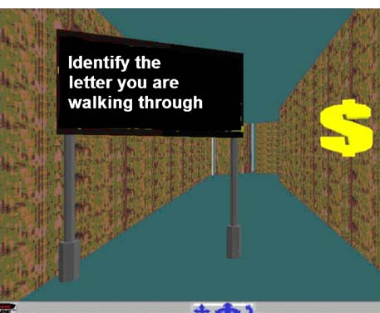
\includegraphics[width=90mm]{images/litreview/dsim1.png}
\caption{Image of dyslexia simulation}
\label{autisim1}
\end{figure}

\begin{figure}[H]
\centering
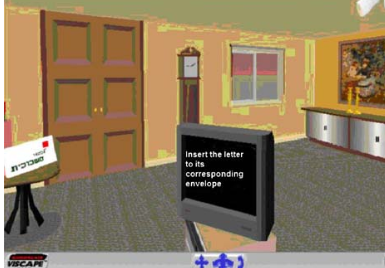
\includegraphics[width=90mm]{images/litreview/dsim2.png}
\caption{Image of dyslexia simulation}
\label{autisim1}
\end{figure}

Results of the study revealed a significant improvement of understanding and awareness in the experimental group whom played the VR simulation.

\begin{figure}[H]
\centering
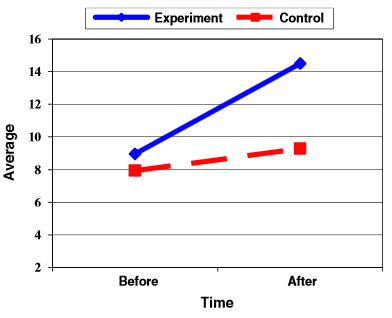
\includegraphics[width=90mm]{images/litreview/dsimresults.png}
\caption{Results of dyslexia simulation}
\label{autisim1}
\end{figure}

Physical disability simulations have been thought to hold disadvantages, potentially lead to pity and misconceptions \cite{dd}, for example the user might take a simulation literally that the experience is exactly what it is like to be all people with, dyslexia for example, rather than a potential representation and experience and understanding that every person is different and will be affected by symptoms in a different way.

A computer simulation may hold an advantage over physical simulations by being possible to depict developed cognitive advantages aspects such as heightened hearing (in the case of visually impaired). In addition computer simulations could highlight thinking differences by visualising the in-game character's thoughts and feelings when approached by various obstacles and these could be used to reduce pity or misconceptions.

In regards to the overall success of simulations, little research has be found to conclude the success or failure of using simulations as a method to raise awareness and understanding apart from \cite{dyslexicsimpar} which also specified "no studies have been made to date, of efforts to increase awareness of the cognitive aspects of the child with learning disability".

\subsection{Autism simulation and tools}

In February 2013 a playable 3D virtual environment depicting sensory difficulties in autism was released. The simulation involved the user navigating a school playground which contained other children whom all looked identical(to represent difficulties with facial recognition). If the user gets too close to the children, visual distortions and high-pitched sounds/screams are played. 

\begin{figure}[H]
\centering
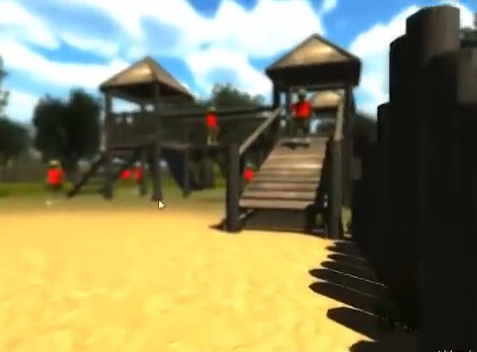
\includegraphics[width=90mm]{images/litreview/autisim1.png}
\caption{Image of playground with no sensory effects}
\label{autisim1}
\end{figure}

\begin{figure}[H]
\centering
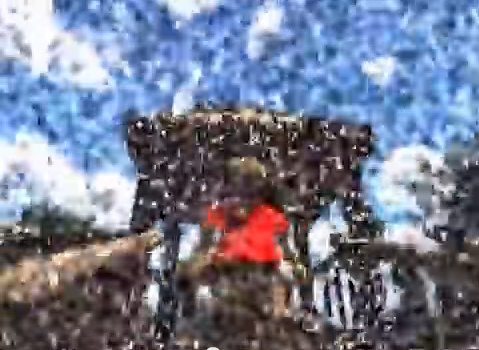
\includegraphics[width=90mm]{images/litreview/autisim2.png}
\caption{Image of playground with sensory effect distortions}
\label{autisim2}
\end{figure}


The simulation from the public was well received and regarded as a good step in increasing awareness and understanding of autism. From those with autism the feedback was mixed with some commenting the portrayal was not an accurate representation of their difficulties whilst for others it was, highlighting the breath of experiences these individuals have and the challenge of the task at hand.

In addition to a playable simulation some autistic individuals have created short videos to demonstrate the impact of sensory problems on their day to day lives and these have been very well received(Gary G. Porter). 
\begin{enumerate}
\item Video simulation of a sensory overload created by a group aiming to use media to help others understand autism: http://www.interactingwithautism.com/section/understanding/sensory/1
\item Video simulation of sensory overload in a supermarket created by an individual with autism: https://www.youtube.com/watch?v=IcS2VUoe12M
\item Autism simulation of a variety of aspects: http://simdis.jisctechdis.ac.uk/Autism/repres.htm
\item Video of sensory overload whilst an individual is walking along a street: https://www.youtube.com/watch?v=plPNhooUUuc
\end{enumerate}

One great benefit of conveying difficulties visually is that it helps obviates to some extent the ever-present language barrier and helping to overcome difficulty for people with autism.  